\documentclass{standalone}

\begin{document}

\section{Sparkling Water Introduction}

Sparkling Water allows users to combine the fast, scalable machine learning algorithms of H2O with the capabilities of Spark. With Sparkling Water, users can drive computation from Scala, R, or Python and use the H2O Flow UI, providing an ideal machine learning platform for application developers.

Spark is an elegant and powerful general-purpose, open-source, in-memory platform with tremendous momentum. H2O is an in-memory application for machine learning that is reshaping how people apply math and predictive analytics to their business problems.

Integrating these two open-source environments provides a seamless experience for users who want to make a query using Spark SQL, feed the results into H2O to build a model and make predictions, and then use the results again in Spark. For any given problem, better interoperability between tools provides a better experience. 

For additional examples, please visit the Sparkling Water GitHub repository at {\url{https://github.com/h2oai/sparkling-water/tree/master/examples}}. 

\subsection{Typical Use Cases}
Sparkling Water excels in leveraging existing Spark-based workflows needed to call advanced machine learning algorithms. We identified three the most common use-cases which are described below. 

\subsubsection{Model Building}
A typical example involves multiple data transformations with help of Spark API, where a final form of data is transformed into H2O frame and passed to an H2O algorithm. The constructed model estimates different metrics based on the testing data or gives a prediction that can be used in the rest of the data pipeline (see Figure~\ref{fig:uc1}).
\begin{figure}[h!]
	\centering
	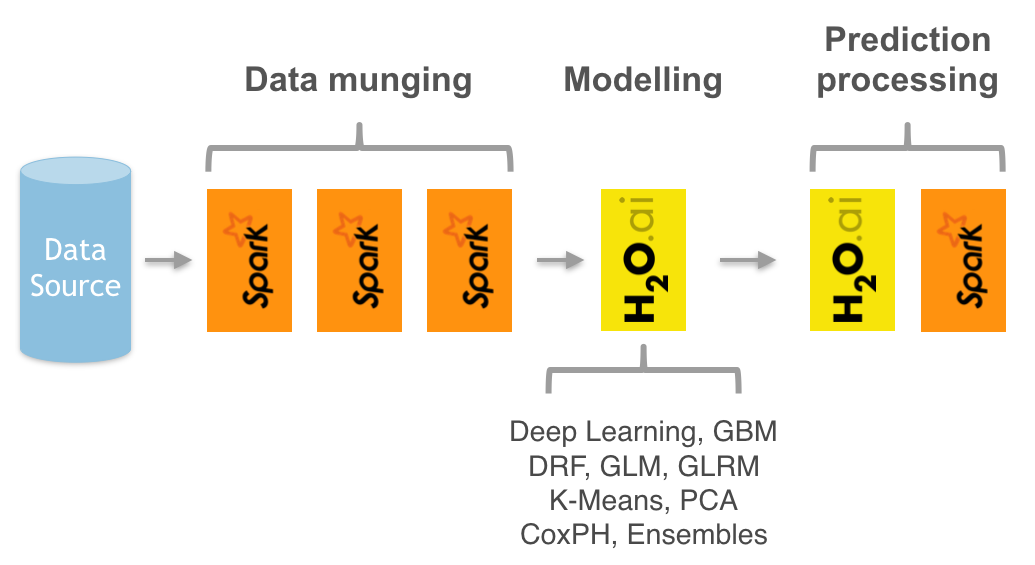
\includegraphics[width=0.9\textwidth]{sw/images/uc1.png}
	\caption{Sparkling Water extends existing Spark data pipeline with advanced machine learning algorithms.}
	\label{fig:uc1} 
\end{figure}

\subsubsection{Data Munging}
Another use-case includes Sparkling Water as a provider of ad-hoc data transformations. Figure~\ref{fig:uc2} shows a data pipeline benefiting from H2O's parallel data load and parse capabilities, while Spark API is used as another provider of data transformations. Furthermore, H2O can be used as in-place data transformer.

\begin{figure}[h!]
	\centering
	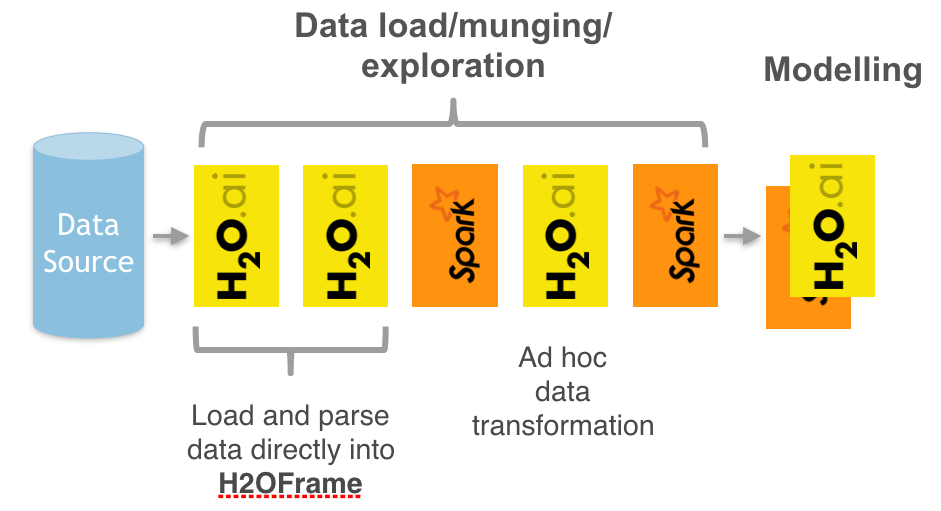
\includegraphics[width=0.9\textwidth]{sw/images/uc2.png}
	\caption{Sparkling Water introduces H2O parallel load and parse into Spark pipelines.}
	\label{fig:uc2} 
\end{figure}

\subsubsection{Stream Processing}
The last use-case depicted on Figure~\ref{fig:uc3} introduces two data pipelines. The first one, called an off-line training pipeline, is invoked regularly (e.g., every hour or every day), utilizes Spark as well as H2O API and provides an H2O model as output. The H2O API allows the model to be exported in a source code form. The second one processes streaming data (with help of Spark Streaming or Storm) and utilizes the model trained in the first pipeline to score the incoming data. Since the model is exported as a code,  the streaming pipeline can be lightweight and independent on H2O or Sparkling Water infrastructure.

\begin{figure}[h]
	\centering
	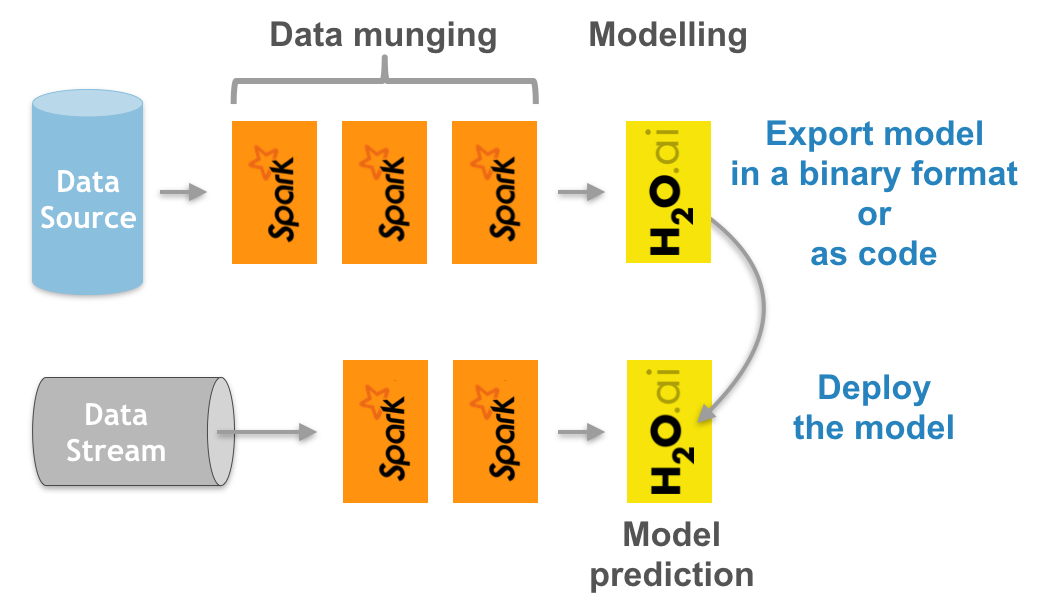
\includegraphics[width=0.9\textwidth]{sw/images/uc3.png}
	\caption{Sparkling Water used as an off-line model producer feeding models into a stream-based data pipeline.}
	\label{fig:uc3} 
\end{figure}

\subsection{Features}

Sparkling Water provides transparent integration for the H2O engine and its machine learning algorithms into the Spark platform, enabling:

\begin{itemize}

 \item Use of H2O algorithms in Spark workflow
 \item Transformation between H2O and Spark data structures
 \item Use of Spark RDDs and DataFrames as input for H2O algorithms
 \item Use of H2OFrames as input for MLlib algorithms
 \item Transparent execution of Sparkling Water applications on top of Spark
\end{itemize}

\subsection{Supported Data Sources}

Currently, Sparkling Water can use the following data source types:

\begin{itemize}

 \item Standard Resilient Distributed Dataset (RDD) API for loading data and transforming it into H2OFrames
 \item H2O API for loading data directly into H2OFrame from file(s) stored on:
  \begin{itemize}
    \item local filesystems
    \item HDFS
    \item S3
    \item HTTP/HTTPS
  \end{itemize}
\end{itemize}

For more details, please refer to the H2O documentation at {\url{http://docs.h2o.ai}}.

\subsection{Supported Data Formats}

Sparkling Water can read data stored in the following formats:

\begin{itemize}

  \item CSV
  \item SVMLight
  \item ARFF
\end{itemize}

For more details, please refer to the H2O documentation at {\url{http://docs.h2o.ai}}.

\subsection{Supported Spark Execution Environments}
Sparkling Water can run on top of Spark in the following ways:
\begin{itemize}
  \item as a local cluster (where the master node is \texttt{local},
\texttt{local[*]}, or \texttt{local-cluster[...]})
  \item as a standalone cluster\footnote{Refer to the Spark standalone documentation
\url{http://spark.apache.org/docs/latest/spark-standalone.html}} 
\item in a YARN environment\footnote{Refer to the Spark YARN documentation \url{http://spark.apache.org/docs/latest/running-on-yarn.html}}

\end{itemize}
\end{document}

